% -----------------------------------------------------------------------------
% ########################
% # PREDLOGA ZA POROCILO #
% ########################
%
% @author Iztok Starc
% @date   3. december 2008
%
\documentclass[a4paper,12pt]{report}

% -----------------------------------------------------------------------------
% ####################################################
% # UPORABA PAKETOV - NASTAVITEV JEZIKA in KODIRANJA #
% ####################################################
\usepackage[slovene]{babel}
\usepackage[utf8]{inputenc}
\usepackage{lmodern}
\usepackage[T1]{fontenc}
\usepackage[sc]{mathpazo}
\linespread{1.05}
\usepackage[T1]{fontenc}

% -----------------------------------------------------------------------------
% ######################################
% # VNOS KLJUCNIH PARAMETROV BESEDILA  #
% ######################################

\newcommand{\naslov}     {Izdelava spletne trgovine Big Shope}
\newcommand{\prviavtor}  {Enej Ravbar}
\newcommand{\prviindeks} {63150236}
\newcommand{\drugiavtor} {Matej Bizjak}
\newcommand{\drugiindeks}{63150053}
\newcommand{\tretjiavtor} {Miha Jamšek}
\newcommand{\tretjiindeks}{63150120}
\newcommand{\kraj}       {Ljubljana}

% -----------------------------------------------------------------------------
% ###################
% # UPORABA PAKETOV #
% ###################
\usepackage[a4paper,left=25mm,right=25mm,top=20mm,bottom=30mm,includehead]{geometry}

\usepackage{graphicx, epsfig}

\usepackage{fancyhdr}

\usepackage[
colorlinks=true, linkcolor=blue, citecolor=red,
%
pdftitle={\naslov},
pdfauthor={\prviavtor, \drugiavtor},
pdfsubject={Poročilo seminarske naloge pri predmetu Elektronsko Poslovanje},
pdfkeywords={spletna prodajalna, PHP, SSL, MySQL}, a4paper, pagebackref=true, unicode]{hyperref}

% -----------------------------------------------------------------------------
\begin{document}

% -----------------------------------------------------------------------------
% ##################
% # NASLOVNA STRAN #
% ##################
\begin{titlepage}
	\begin{center}
	{UNIVERZA V LJUBLJANI\\[10pt] 
	FAKULTETA ZA RAČUNALNIŠTVO IN INFORMATIKO}

	\vspace{65mm}

	{\Large\textbf{\naslov}}

	\vspace{10mm}

	{\large Poročilo seminarske naloge pri predmetu\\[10pt] Elektronsko poslovanje}

	\vfill
	\vspace{60mm}

\hspace{20mm}
\begin{minipage}[t]{70mm}
	{\bf Študenti}\\
	{\prviavtor} ({\prviindeks})\\ 
	{\drugiavtor} ({\drugiindeks})\\
	{\tretjiavtor} ({\tretjiindeks})
\end{minipage}
%\hfill
\begin{minipage}[t]{50mm}
	{\bf Mentor}\\
	David Jelenc
\end{minipage}
%\hspace{20mm}

	\vspace{35mm}

	{	\kraj, \today}
	\end{center}
\end{titlepage}

% -----------------------------------------------------------------------------
% ##################
% # KAZALO VSEBINE #
% ##################

\tableofcontents

% -----------------------------------------------------------------------------
% ############
% # POVZETEK #
% ############
%\begin{abstract}
%\end{abstract}

% -----------------------------------------------------------------------------
% ##################
% # UVOD DOKUMENTA #
% ##################
\chapter{Uvod}

Naloga seminarske naloge je bila izdelava varne spletne trgovine. Pri tem smo uporabili Linux operacijski sistem, na katerem teče Apache strežnik za posredovanje PHP datotek, MySQL podatkovno bazo za hranjenje podatkov, SSL/TLS protokol za posredovanje varne vsebine, X.509 za identifikacijo osebja ter VueJS, jQuery in BootStrap za prikaz vsebine na odjemalcu. Izdelali smo tudi Android aplikacijo ki preko REST storitve komunicira z strežnikom.

% -----------------------------------------------------------------------------
% ###################
% # JEDRO DOKUMENTA #
% ###################

% -----------------------------------------------
\chapter{Navedba realiziranih storitev}

Implementirali smo naslednje razširjene storitve:

\begin{itemize}  
\item Vodenje dnevnika: vodimo tri dnevnike: dnevnik za prodajalca, dnevnik za administratorja ter splošni dnevnik - vsak se zapisuje v svojo tekstovno datoteko.
\item Registracija strank s potrditvenim e-mailom: Ob registraciji stranke, bodisi ko se registrira sama, bodisi ko jo registrira prodajalec, se pošlje potrditveni e-mail na posredovani račun.
\item Uporabniški vmesnik
\item Predstavitev artiklov s slikami. Slike se hranijo na datotečni sistem, njihovi metapodatki pa v tabelo v podatkovno bazo.
\item Android aplikacija: v aplikaciji stranka lahko anonimno pregleduje izdelke, če se prijavi pa si lahko ogleduje svoj profil ter ga posodablja
\end{itemize}



% -----------------------------------------------
\chapter{Podatkovni model}

\begin{figure}[htbp]
\begin{center}
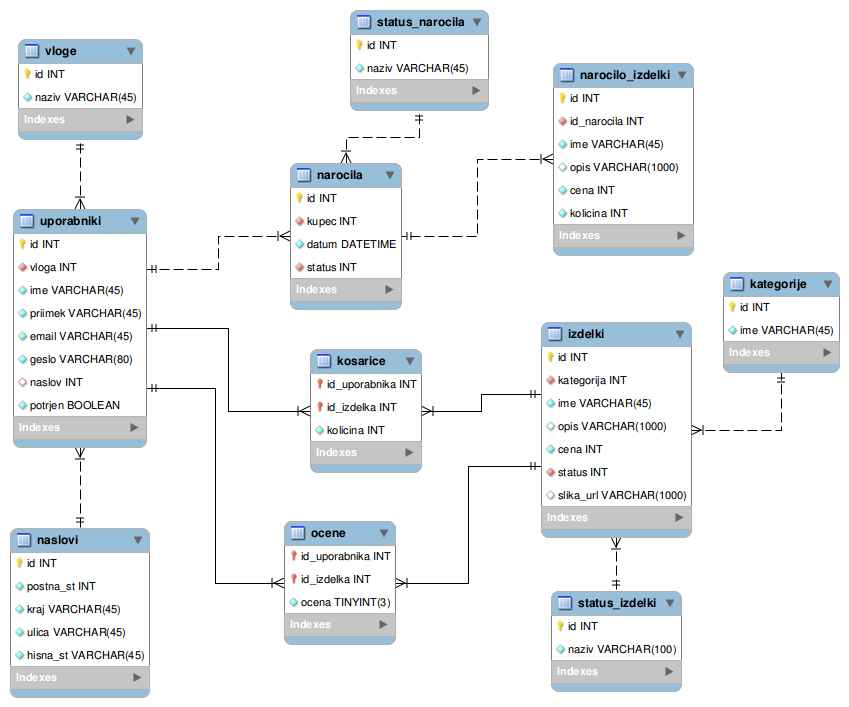
\includegraphics[scale=0.32]{err_diagram.png}
\caption{E-R diagram}
\label{Tekstovni dendrogram}
\end{center}
\end{figure}

TODO: opis

% -----------------------------------------------
\chapter{Varnost sistema}

Trgovina omejuje dostop preko protokola HTTP za veliko večino strani, vse ostale zahteve so dostopne samo preko HTTPS, pri čemer trgovina sama skrbi za ustrezno preklapljanje. Stranke se lahko registrirajo in tako koristijo funkcionalnosti nakupa, pri čemer se njihovo geslo enosmerno kriptira, njihov elektronski naslov pa se preveri, tako, da je na ta naslov poslano sporočilo, v katerem je povezava, ki ob obisku dokonča aktivacijo računa. Ob registraciji mora stranka tudi izpolniti reCaptcha test, ki preveri ali je klient oseba.

Vsak vnos podatkov iz strani odjemalca se filtrira, kjer so prečiščeni vsi posebni znaki - to nas brani pred XSS napadi in vsak vnos podatkov v podatkovno bazo uporablja parametriziran SQL niz, kar preprečuje SQL injection napade. Osebje, torej administrator in prodajalci se prijavljajo na posebni povezavi, ki zahteva od klienta, da ta posreduje svoj veljavni X.509 certifikat, ki dokazuje njegovo istovetnost ter, da se prijavi z istimi podatki, kot so podani v certifikatu. Nadalje, vsak REST API prvo preveri ali ima trenutno prijavljen uporabnik sploh pravice za dostop do tega API, nakar izvede svoj klic, če jih ima, ali pa zavrne dostop.

% -----------------------------------------------
\chapter{Izjava o avtorstvu seminarske naloge}

Spodaj podpisani \textit{\prviavtor}, vpisna številka \textit{\prviindeks}, sem (so)avtor seminarske naloge z naslovom \textit{\naslov}. S svojim podpisom zagotavljam, da sem izdelal ali bil soudeležen pri izdelavi naslednjih sklopov seminarske naloge:
\begin{itemize}
    \item Vzorčni sklop 1
	\item Vzorčni sklop 2
\end{itemize}

Podpis: {\prviavtor}, l.r.

\newpage

Spodaj podpisana \textit{\drugiavtor}, vpisna številka \textit{\drugiindeks}, sem (so)avtor seminarske naloge z naslovom \textit{\naslov}. S svojim podpisom zagotavljam, da sem izdelal ali bil soudeležen pri izdelavi naslednjih sklopov seminarske naloge:
\begin{itemize}
    \item TODO
    \item Vzorčni sklop 2
\end{itemize}

Podpis: {\drugiavtor}, l.r.

\newpage

Spodaj podpisana \textit{\tretjiavtor}, vpisna številka \textit{\tretjiindeks}, sem (so)avtor seminarske naloge z naslovom \textit{\naslov}. S svojim podpisom zagotavljam, da sem izdelal ali bil soudeležen pri izdelavi naslednjih sklopov seminarske naloge:
\begin{itemize}
    \item Zaledni del za upravljanje strank, prodajalcev in administratorja
    \item Zaledno upravljanje s slikami
    \item Verifikacija strankinega elektronskega naslova
    \item Zaledni del za upravljanje izdelkov
    \item Android aplikacija
    \item Vodenje dnevnika za prodajalca in administratorja
    \item Izdelava certifikatne agencije in certifikatov
\end{itemize}

Podpis: {\tretjiavtor}, l.r.

% -----------------------------------------------
\chapter{Dodatno vzorčno poglavje}

Besedilo poglavja.

\section{Dodatni vzorčni odsek ena}

Besedilo odseka.

\section{Dodatni vzorčni odsek dva}

Besedilo odseka.

\section{Dodatni vzorčni odsek tri}

Besedilo odseka.

\begin{table}[htb]
 \centering
 \begin{tabular}{c || c}
  \textbf{N} & Vsebina\\ \hline\hline
  1 & Vrstica 1\\        \hline
  2 & Vrstica 2\\        \hline
  ... & ... \\
\end{tabular}
\caption{Tabela vrednosti vzorcev}
\label{tab:1}
\end{table}

Besedilo odseka.

\begin{figure}[htb]
	\centering
	\includegraphics[width=13cm]{img/vzorec.jpg}
	\caption{Slika določenega vzorca}
\label{fig:1}
\end{figure}

Besedilo odseka.

% -----------------------------------------------------------------------------
% #######################
% # ZAKLJUCEK DOKUMENTA #
% #######################
\chapter{Zaključek}

Zaključek.

% -----------------------------------------------------------------------------
% ##############
% # LITERATURA #
% ##############
\begin{thebibliography}{99}
\addtocounter{chapter}{1}
\addcontentsline{toc}{chapter}{\protect\numberline{\thechapter}Literatura}
\addtocontents{toc}{\protect\vspace{15pt}}

\bibitem{bib:ref} Yank K. \emph{Build Your Own Database-Driven Website Using PHP \& MySQL}. SitePoint, 2003. ISBN-10: 0-957-92181-0.

\bibitem{bib:ref1} Michele D.; Jon P. \emph{Learning PHP and MySQL}. O'Rielly, 2006. ISBN-10: 0-596-10110-4.

\bibitem{bib:ref2} Tim C.; Joyce P.; Clark M. \emph{PHP5 and MySQL Bible}. Wiley Publishing, Inc., 2004. ISBN-10: 0-7645-5746-7

\bibitem{bib:LinuxCommandReference} Red Hat Software inc. \emph{Linux Complete Command Reference}. Sams Publishing, 1997. ISBN-10: 0-672-31104-6.

\bibitem{bib:IPsecHowTo1} Ralf Spennberg. \emph{IPsec HOWTO} (online). 2003. (citirano \today). Dostopno na naslovu:
\url{http://www.ipsec-howto.org/t1.html}

\end{thebibliography}

% -----------------------------------------------------------------------------
% ###########
% # DODATEK #
% ###########

 \appendix

\chapter{Naslov dodatka}
{\it Po potrebi.}

\end{document}
